\hypertarget{hoare-logic-and-its-mechanization}{%
\section{Hoare Logic and its
Mechanization}\label{hoare-logic-and-its-mechanization}}

\begin{itemize}
\tightlist
\item
  means to prove the Hoare triple \{ P \} C \{ Q \} valid
\item
  Hoare logic is a logic for obtaining valid Hoare triples by purely
  deductive reasoning, that is, by mathematical proof
\item
  deductive reasoning means successively applying inference rules to
  axioms and already obtained conclusions to obtain new conclusions
\item
  such proofs usually are extremely long and boring
\item
  and therefore must be performed as automatically as possible (by
  programs that are by themselves reliable \ldots{})
\item
  but: proof problem is undecidable in the general case
\end{itemize}

\hypertarget{weakest-preconditions}{%
\subsection{Weakest Preconditions}\label{weakest-preconditions}}

\begin{itemize}
\tightlist
\item
  given a command C and a postcondition Q
\item
  given a prestate, the following three things may happen:

  \begin{enumerate}
  \def\labelenumi{\alph{enumi})}
  \tightlist
  \item
    execution of C terminates in a poststate that satisfies Q
  \item
    execution of C does not terminate
  \item
    execution of C terminates in a poststate that satisfies $\neg$Q
  \end{enumerate}
\item
  let w be the set of all prestates from a) and b) together
\item
  a weakest precondition W for C and Q is a boolean formula that
  describes exactly this set
\item
  obviously, weakest preconditions are not unique, since with W $\in$ wp(C,
  Q), for instance, W $\land$ true $\in$ wp(C, Q)
\item
  but clearly, all W $\in$ wp(C, Q) are equivalent
\end{itemize}

\begin{tcolorbox}[colback=red!5!white,colframe=red!75!black]
$\models$ { P } C { Q } is equivalent to $\models$ P $\Rightarrow$ wp(C, Q)
\end{tcolorbox}

\hypertarget{rules-of-inference}{%
\subsection{Rules of Inference}\label{rules-of-inference}}

\begin{itemize}
\tightlist
\item
  let f, f 1 , \ldots{}, f n be boolean formulas (here assertions or
  Hoare triples), n $\geqslant$ 0
\item
  an inference rule is a syntactic construct of the following form:
\end{itemize}

\begin{figure}[H]
\centering
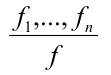
\includegraphics[width=50px]{figures/inferenceRule.png}
\caption{Inference Rule}
\end{figure}

\begin{itemize}
\tightlist
\item
  f\_1 , \ldots{}, f\_n are called premises or hypotheses
\item
  f is called conclusion
\item
  if there are no premises (n = 0), the rule is called an axiom
\item
  the conclusion f is valid, if all hypotheses are valid
\end{itemize}

\hypertarget{skip-axiom}{%
\subsubsection{Skip Axiom}\label{skip-axiom}}

\begin{figure}[H]
\centering
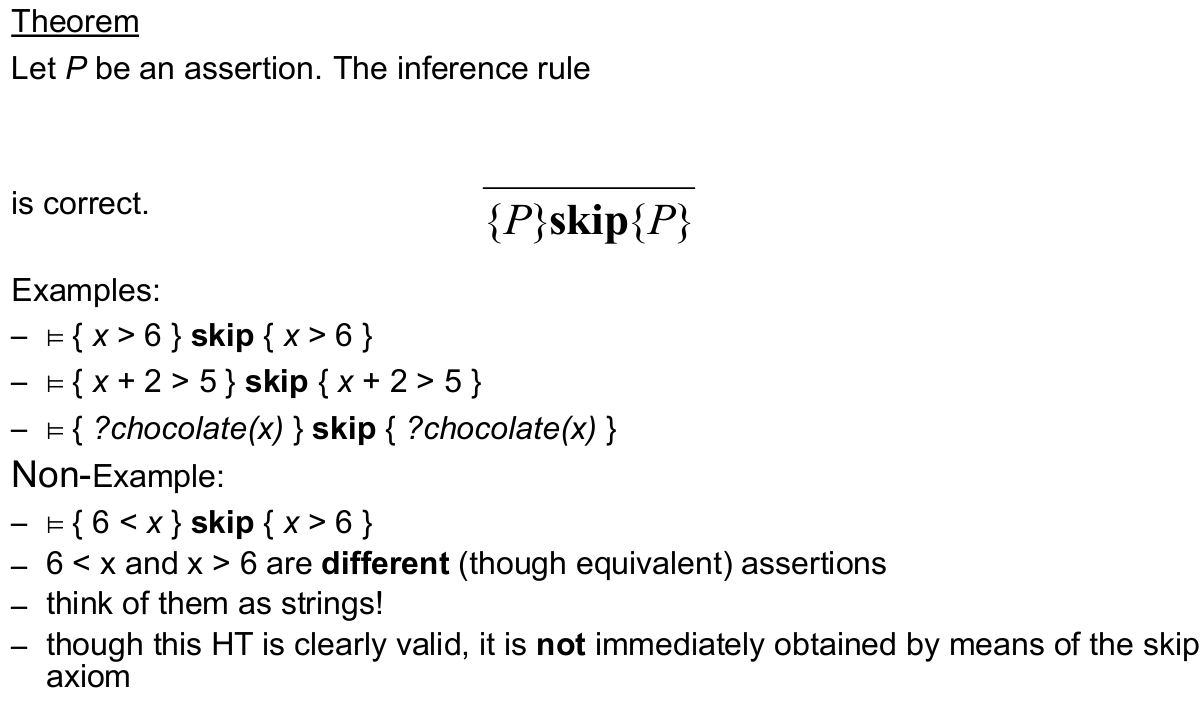
\includegraphics[width=0.7\textwidth]{figures/skipAxiom.png}
\caption{Skip Axiom}
\end{figure}

\begin{tcolorbox}[colback=red!5!white,colframe=red!75!black]
$\{ 6 < x \}$ not equal $\{ x > 6 \}$
\end{tcolorbox}

\clearpage
\hypertarget{rule-of-consequence}{%
\subsection{Rule of Consequence}\label{rule-of-consequence}}

the RoC is of utmost importance:

\begin{itemize}
\tightlist
\item
  it provides the interface between Hoare logic, concerned with
  programming, and „ordinary`` mathematics
\item
  \ldots{} or in other words, it allows to plug in ordinary mathematics
  into Hoare logic
\end{itemize}

\begin{figure}[H]
\centering
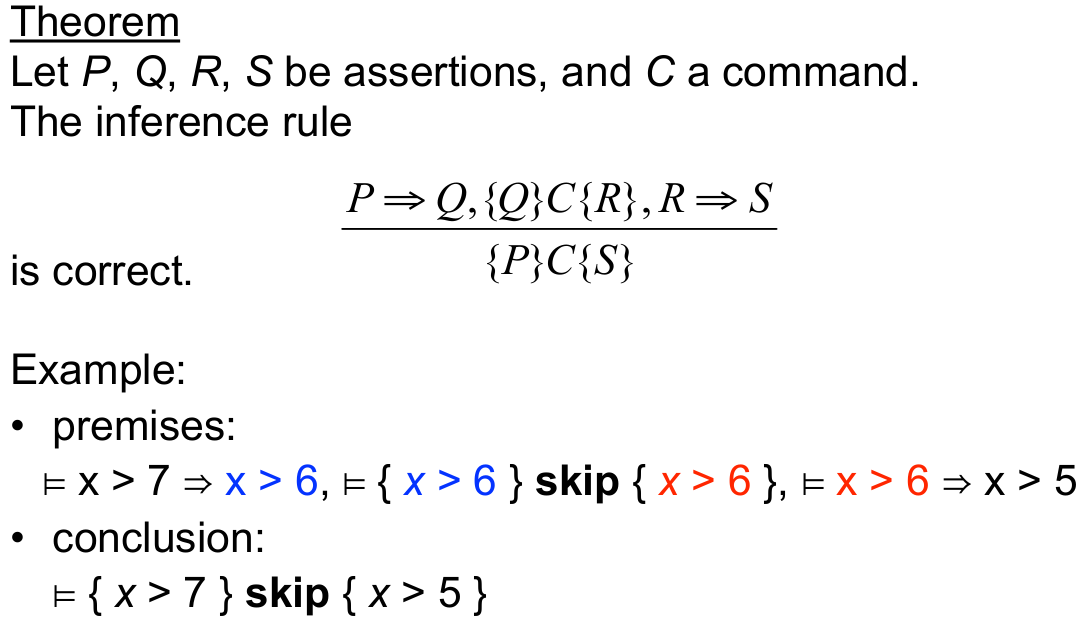
\includegraphics[width=0.7\textwidth]{figures/rulesOfConsquence.png}
\caption{Rules of Consequence}
\end{figure}

We now write this proof of $\models$ \{ x \textgreater{} 7 \} skip \{ x
\textgreater{} 5 \} more concisely and much closer to normal programming
as

\begin{lstlisting}
{ x > 7 }
{ x > 6 }
skip
{ x > 6 }
{ x > 5 }
\end{lstlisting}

\begin{itemize}
\tightlist
\item
  premises:

  \begin{itemize}
  \tightlist
  \item
    we read lines 1 and 2 as implication $\Rightarrow$ (first premise of RoC)
  \item
    we read lines 2 --- 4 as HT (second premise of RoC)
  \item
    we read lines 4 and 5 as implication $\Rightarrow$ (third premise of RoC)
  \end{itemize}
\item
  conclusion:

  \begin{itemize}
  \tightlist
  \item
    we read lines 1 --- 5 as HT (conclusion of RoC)
  \end{itemize}
\end{itemize}

\clearpage
\hypertarget{general-proof-procedure}{%
\subsection{General Proof Procedure}\label{general-proof-procedure}}

\begin{itemize}
\tightlist
\item
  To prove \{P\} C \{Q\}, we start with the postcondition Q, go
  backwards over the command C to determine a precondition R such that
  the HT \{R\} C \{Q\} is valid, and construct the implication P
  -\textgreater{} R.
\item
  This implication is called a verification condition (VC).
\item
  If this VC is valid, then the original HT \{P\} C \{Q\} is valid too.
\item
  this process can be mechanized, that is, performed fully automatically
  be means of a - computer
\item
  there might be many possible preconditions, which one do we choose?
\item
  we always choose the syntactically weakest precondition
\item
  that is, we can assume as little as possible
\end{itemize}

\begin{lstlisting}
Example
{ x > 7 } -- given precondition P
{ x > 5 } -- compute precondition R
skip  
-- go backwards over the command C
{ x > 5 } -- start here with given postcondition Q now construct VC P $\Rightarrow$ R, 
          -- that is, "x > 7 $\Rightarrow$ x > 5"
\end{lstlisting}

\hypertarget{computing-preconditions-and-software-engineering}{%
\subsubsection{Computing Preconditions and Software
Engineering}\label{computing-preconditions-and-software-engineering}}

\begin{itemize}
\tightlist
\item
  looks strange in the first moment to start with the postcondition to
  arrive at the precondition
\item
  but: \textbf{the postcondition describes the actual task of the
  program and is thus given}
\item
  the precondition will be determined to find out under which
  circumstances the postcondition can be achieved
\item
  happily, determining preconditions from postconditions is much simpler
  than the other way round
\item
  thus, determining VCs (via computing preconditions) can be done
  automatically by a tool called a \textbf{verification condition
  generator}
\item
  the VCs can then (hopefully automatically) be discharged (proved
  valid) by a second tool called a theorem prover
\end{itemize}

\hypertarget{textual-substitution}{%
\subsubsection{Textual Substitution}\label{textual-substitution}}

This is an operation that essentially can be performed by means of
search and replace of a text editor, and thus can be implemented on a
machine.

\begin{lstlisting}
x[x<-z+2] yields (z + 2)
-- or
y[x<-z+2] yields y
-- [x<-z+2] this will replace all x with z+2
\end{lstlisting}

\hypertarget{assignment-axiom}{%
\subsection{Assignment Axiom}\label{assignment-axiom}}

\begin{itemize}
\tightlist
\item
  The assigning command can be seen as something like renaming an
  expression in the precondition.
\item
  You take the expression in the execution part and assign this defition
  of the variable (in the execution part) to the same variable in the
  precondition.
\item
  If the new precondition can still meet the postcondition (after
  execution), the Hoare is valid.
\end{itemize}

\begin{figure}[H]
\centering
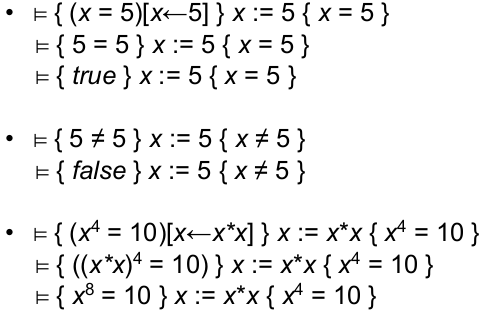
\includegraphics[width=0.5\textwidth]{figures/assigningAxiom.png}
\caption{Assignment Axiom Examples}
\end{figure}

\hypertarget{composition-command}{%
\subsection{Composition Command}\label{composition-command}}

The composition command is used to do one or more things one after the
other.

\begin{figure}[H]
\centering
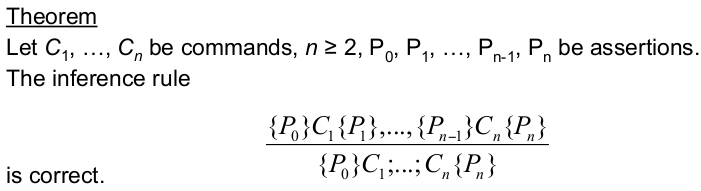
\includegraphics[width=0.7\textwidth]{figures/compositionrule.png}
\caption{Composition Rule}
\end{figure}

\begin{figure}[H]
\centering
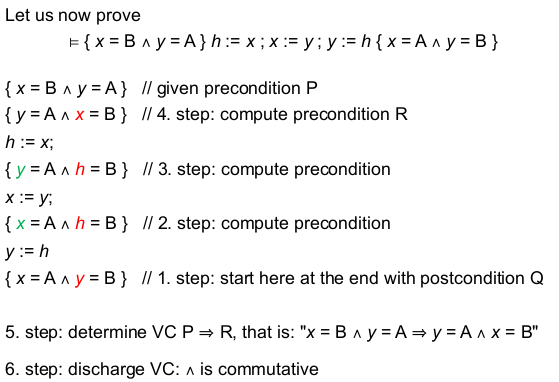
\includegraphics[width=0.5\textwidth]{figures/compositionExample.png}
\caption{Composition Example}
\end{figure}

\hypertarget{example-strange-swap}{%
\subsubsection{Example Strange Swap}\label{example-strange-swap}}

\begin{figure}[H]
\centering
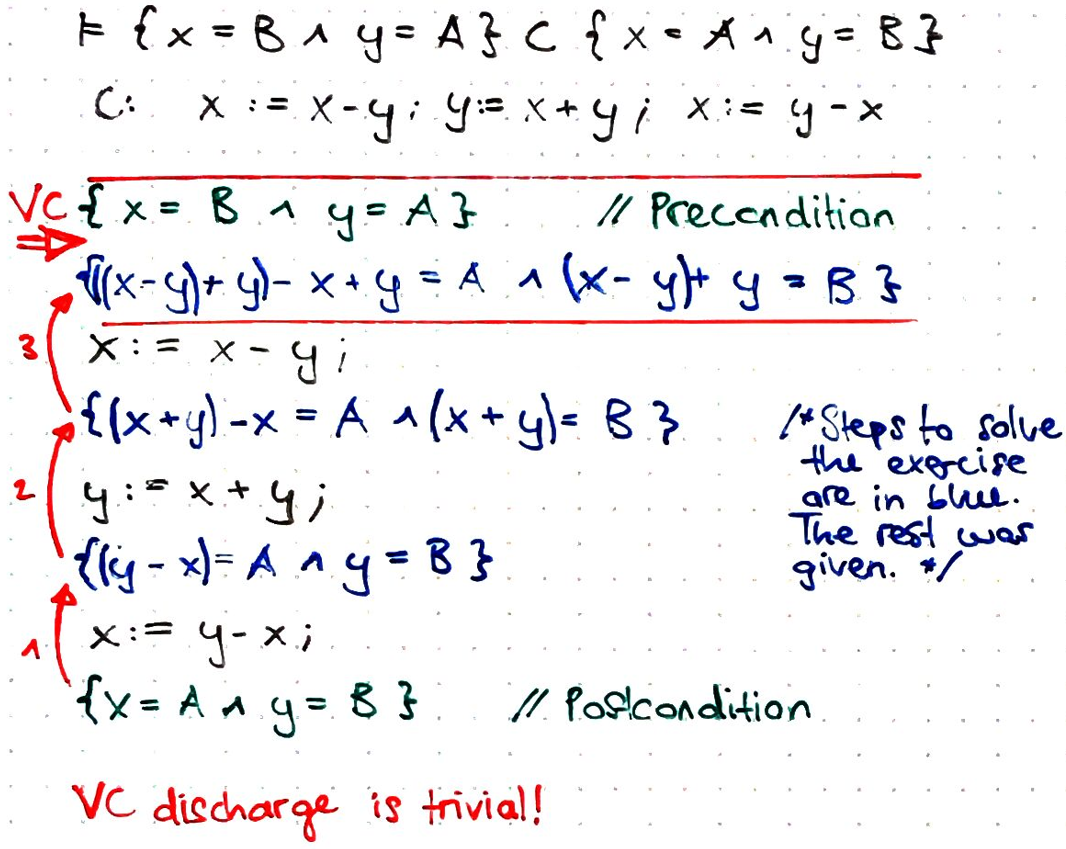
\includegraphics[width=0.6\textwidth]{figures/exampleStrangeSwap.png}
\caption{Strange Swap Example}
\end{figure}

\hypertarget{conditional-rule}{%
\subsection{Conditional Rule}\label{conditional-rule}}

\begin{figure}[H]
\centering
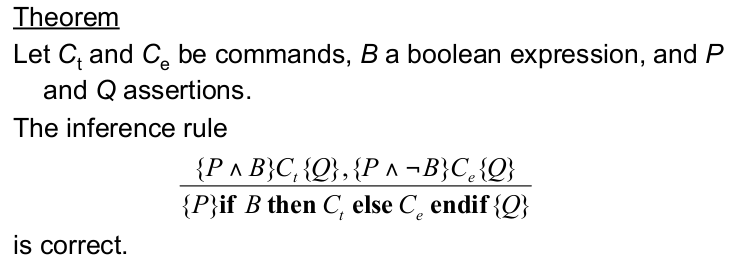
\includegraphics[width=0.6\textwidth]{figures/conditionalRule.png}
\caption{Conditional Rule}
\end{figure}

\begin{figure}[H]
\centering
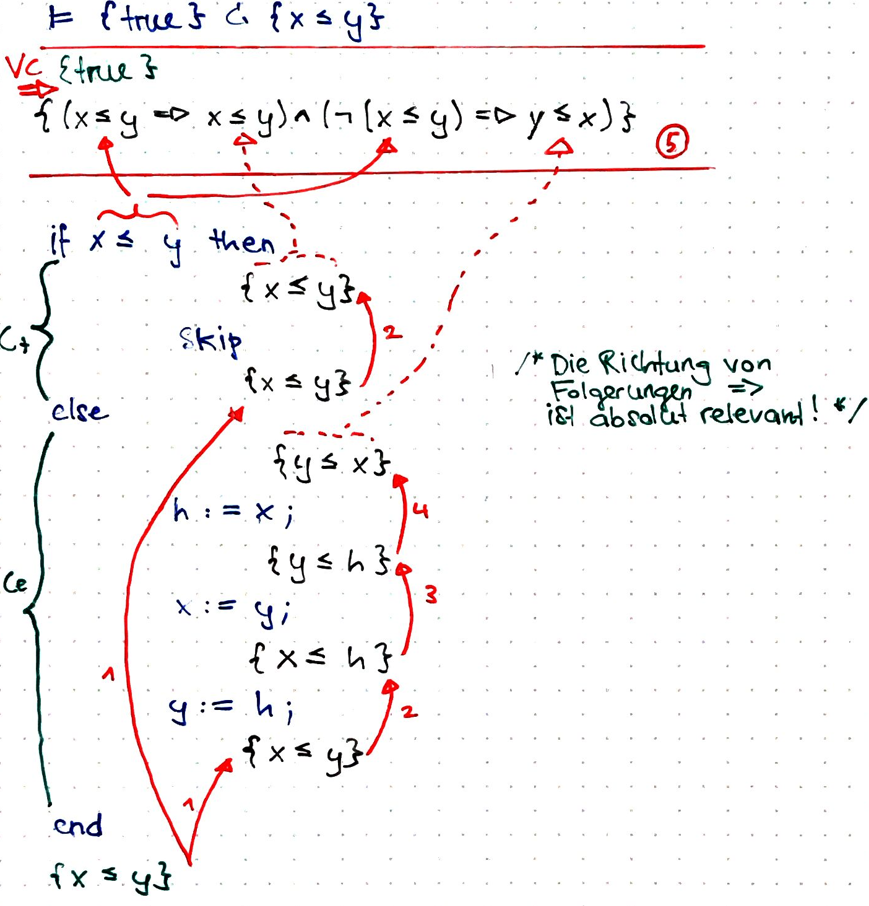
\includegraphics[width=0.8\textwidth]{figures/exampleConditional.png}
\caption{Conditional Rule Example}
\end{figure}

\clearpage